% !TEX root = D:\Users\Ignacio\Documentos\Escuela\CC3002 - Metodologías de Diseño y Programación\apunte-y-ejercicios\src\latex\Apunte.tex
\section{Ejercicios}
  \begin{Exercise}[title={Publicaciones}]
    Para este ejercicio se considerarán personas, autores y obras, y se modelará una 
    estructura de clases para representar las relaciones entre ellas.

    \begin{enumerate}
      
      \item Considere la siguiente implementación de un autor:
        \begin{minted}{java}
          class Author {
            String name;
            int money;

            Title[] publishedTitles = new Title[8];
            int publishedTitlesCount = 0;
            Title[] boughtTitles = new Title[8];
            int boughtTitlesCount = 0;

            Author(String name, int money) {
              this.name = name;
              this.money = money;
            }

            void write(String name, String content, Title title) {
              title.content += content;
            }

            void publish(Title title, int price) {
              title.price = price;
              if (publishedTitlesCount == publishedTitles.length) {
                Title[] auxArr = new Title[publishedTitles.length * 2];
                for (int idx = 0; idx < publishedTitles.length; idx++) {
                  auxArr[idx] = publishedTitles[idx];
                }
                publishedTitles = auxArr;
              }
              publishedTitles[publishedTitlesCount++] = title;
            }

            void distribute(Title title, Store store) {
              store.addTitle(title);
            }

            void buy(Title title, Store store) {
              if (money >= title.price) {
                store.money += title.price;
                if (boughtTitlesCount == boughtTitles.length) {
                  Title[] auxArr = new Title[boughtTitles.length * 2];
                  for (int idx = 0; idx < boughtTitles.length; idx++) {
                    auxArr[idx] = boughtTitles[idx];
                  }
                  boughtTitles = auxArr;
                }
                boughtTitles[boughtTitlesCount++] = title;
              }
            }
          }
        \end{minted}

        Juzgue si esta implementación cumple con los \textit{principios SOLID} y, en caso
        de que viole alguno, especifique cuál y proponga una solución (no es necesario 
        que la programe).

      \item Considere ahora que un autor es solamente una persona que ha publicado alguna 
        obra.
        ?`Cambia esto de alguna forma la implementación anterior?

        \textit{Hint: ?`Qué tanto diferirían una clase \texttt{Author} de una clase 
        \texttt{Person}?}
      
      \item Una persona puede escribir múltiples tipos de trabajos, en particular 
        \textbf{novelas}, \textbf{cuentos}, \textbf{\textit{papers}} y \textbf{libros 
        científicos}.

        Tanto las novelas como los cuentos son \textbf{obras literarias}, los 
        \textit{papers} y libros científicos son \textbf{publicaciones científicas} y las 
        novelas y libros científicos son \textbf{Libros}, y los 4 son \textbf{trabajos 
        escritos}.

        Proponga un esquema de clases para representar esta estructura (basta con un 
        diagrama simple).

      
      \item Diremos que una \textbf{revista científica} es una recopilación de 
        \textit{papers} y una \textbf{antología} es un conjunto de cuentos.
        Una antología es una obra literaria y un libro, mientras que una revista 
        científica es una publicación científica.
        Ambas son obras escritas.

        Modifique el diagrama de su respuesta anterior para incluir estos nuevos tipos.
      
      \item Lo último será definir dos nuevos tipos de entidades, las \textbf{editoriales}
        y las \textbf{tiendas}.

        Una \textbf{editorial} se encarga de publicar las obras de un autor y 
        distribuirlas a tiendas.
        Las editoriales \textbf{siempre} se especializan en un tipo de obra, siendo estas
        publicaciones científicas u obras literarias.

        Por otro lado, una \textbf{tienda} compra obras a las editoriales, pero solamente 
        si son libros o revistas.
        Además, una tienda puede o no especializarse en un tipo particular de publicación
        (literaria o científica).

        Bosqueje las clases necesarias para representar este comportamiento y los métodos 
        necesarios para que una editorial publique una obra y una tienda compre de acuerdo 
        a las restricciones que se impusieron en los párrafos anteriores (esto puede ser 
        en \textit{Java}, pseudo-código o como un diagrama pero deben especificarse 
        claramente los tipos de los objetos involucrados en el proceso).
    \end{enumerate}
  \end{Exercise}

  \begin{Exercise}[title={Algebra vectorial}]
    \begin{enumerate}
      \item El largo (o norma) de un vector \(\mathbf{v}\) es la distancia de dicho vector 
        respecto al origen del sistema de coordenadas y se denota como \(||\mathbf{v}||\).
        La norma de un vector se define como:

        \[  
          ||\mathbf{v}|| = 
            \sqrt{\mathbf{v}_0^2 + \mathbf{v}_1^2 + \cdots + \mathbf{v}_n^2 }
        \]

        Implemente el método \mintinline{java}{double getLength()} que calcule el largo de
        un vector de dimensión \(n\). 

      \item Un \textit{vector cero} es un vector especial de largo arbitrario que cumple 
        la propiedad de que sumarlo con cualquier otro vector da el mismo vector.
        Formalmente, sea un vector \(\mathbf{v}\) de dimensión arbitraria y el vector 
        \(\mathbf{0}\) de dimensión indefinida: se dice que \(\mathbf{0}\) es un vector 
        cero ssi \(\mathbf{v} + \mathbf{0} = \mathbf{v},\ \forall \mathbf{v}\).

        Programe una clase \texttt{ZeroVector} que implemente dicha funcionalidad al ser 
        sumado con cualquier otro vector.
      
      \item Agregue un método (en las clases que estime necesarias) 
        \mintinline{java}{boolean isZeroVector()} que retorne \mintinline{java}{true} si
        el objeto es un vector cero y \mintinline{java}{false} en caso contrario.
        Note que un objeto de clase \texttt{VectorND} también podría ser un vector cero.

      \item Dos vectores \(\mathbf{a}\) y \(\mathbf{b}\) se dicen opuestos si 
        \(\forall i \in \mathbb{Z}\) 
        se cumple que \(\mathbf{a}_i = -\mathbf{b}_i\).
        Extienda la clase \texttt{VectorND} con un método 
        \mintinline{java}{boolean isOppositeTo(VectorND)} que retorne 
        \mintinline{java}{true} si los vectores son opuestos y \mintinline{java}{false} 
        en caso contrario.
      
      \item El \textit{producto punto} entre 2 vectores \(\mathbf{a}\) y \(\mathbf{b}\) de 
        dimensiones \(m\) y \(n\) respectivamente, con \(m \leq n\) se define como:
        \[
          \mathbf{a} \cdot \mathbf{b} = \mathbf{a}_1 \mathbf{b}_1 
            + \mathbf{a}_2 \mathbf{b}_2 + \cdots + \mathbf{a}_m \mathbf{b}_m
        \]

        Implemente el método \mintinline{java}{double dotProduct(VectorND)} que calcule
        el producto punto entre 2 vectores.
      
      \item El \textit{producto cruz} es una operación entre dos vectores de 3 dimensiones 
        que da como resultado un nuevo vector perpendicular a ambos.
        Se define el producto cruz entre dos vectores \(\mathbf{a}\) y \(\mathbf{b}\) 
        como:

        \[  
          \mathbf{a} \times \mathbf{b} = \left(
            \mathbf{a}_2 \mathbf{b}_3 - \mathbf{a}_3 \mathbf{b}_2,\,
            \mathbf{a}_3 \mathbf{b}_1 - \mathbf{a}_1 \mathbf{b}_3,\,
            \mathbf{a}_1 \mathbf{b}_2 - \mathbf{a}_2 \mathbf{b}_1
            \right)
        \]

        Cree un método \mintinline{java}{Vector3D crossProduct(Vector3D)} que haga este 
        cálculo.
    \end{enumerate}
  \end{Exercise}

  \begin{Exercise}[title={Estructura \textit{Half-edge}}]
    Una \textit{estructura Half-edge} establece una relación entre los componentes que 
    describen mallas de polígonos (i.e. vértices, arcos y polígonos) 
    ampliamente usados en la \textit{computación gráfica}.

    La ventaja de utilizar esta estructura sobre otras es que permite responder varias 
    preguntas comunes respecto a los polígonos que se representan con esta estructura:

    \begin{itemize}
      
      \item ?`Qué arcos están conectados a un vértice?
      \item ?`Qué polígonos están conectados a un vértice?
      \item ?`Qué vértices están conectados a un polígono? 
    \end{itemize}

    utilizando una cantidad constante de memoria.

    \begin{note}
      Una estructura \textit{Half-edge} no puede utilizarse para representar 
      \textit{superficies no orientables} ni superficies con topologías 
      \textit{non-manifold}.
    \end{note}

    Esta estructura obtiene su nombre ya que representa cada arco de una figura como 2 
    semi-arcos con orientación anti-horaria.

    A continuación se plantean los requisitos para implementar esta estructura:

    \begin{enumerate}
      
      \item Un \textit{Half-edge} es una línea que tiene un vértice de origen y uno de 
        destino, puede estar conectado a 0 ó 1 polígonos y todo \textit{Half-edge} está 
        conectado a otro \textit{Half-edge} asociado a los mismos vértices pero en 
        sentido contrario, a este último se le llama pareja (de ahí el nombre 
        \textit{\textbf{Half}-edge}).
        Un arco se define como un par de \textit{Half-edges} que sean parejas entre sí.

        Defina las clases y constructores necesarios para representar esta estructura 
        considerando vértices de \(n\) dimensiones de modo que cada vértice y polígono 
        referencie a lo más a uno de sus \textit{Half-edges}.

        Para simplificar los problemas siguientes es recomendable que agregue un campo 
        \texttt{String id} a cada clase para luego poder imprimir en pantalla el 
        \textit{id} de cada objeto.
      
      \item Cree un método que indique si dos vértices son adyacentes (i.e. que están 
        unidos por un arco).
      
      \item Agregue un método que indique si dos polígonos son adyacentes (i.e. tienen al 
        menos un arco en común).
        
      \item Agregue un método que permita definir el \textit{Half-edge} siguiente de otro.
        Un ejemplo de uso de este método podría ser:
        
        \begin{minted}{java}
          halfEdge1.setNext(halfEdge2);
        \end{minted}

      \item Implemente un método que permita recorrer los arcos conectados a un vértice en 
        sentido antihorario e imprima en pantalla cada uno de los arcos recorridos, de 
        forma tal que un mismo \textit{Half-edge} no sea recorrido más de una vez.
      
      \item Escriba un método que permita recorrer los arcos alrededor de un polígono en 
        sentido antihorario y los imprima en pantalla, nuevamente, asegúrese de que cada 
        \textit{Half-edge} no sea recorrido más de una vez.
      
      \item Cree un método para añadir un arco entre dos vértices. 
        Tenga en cuenta que agregar un nuevo arco implicará cambiar las referencias de 
        algunos de los semi-arcos de los vértices para respetar el invariante de que el 
        recorrido debe hacerse siempre en sentido horario.
        Para esto último puede tomar como referencia la figura \ref{fig:he-add-edge}, note
        que al agregar el nuevo arco, el semi-arco \textbf{a} pasa a apuntar al semi-arco
        \textbf{i} y el semi-arco \textbf{c} pasa a apuntar a \textbf{j} formándose un 
        nuevo polígono.
        \begin{figure}[ht!]
          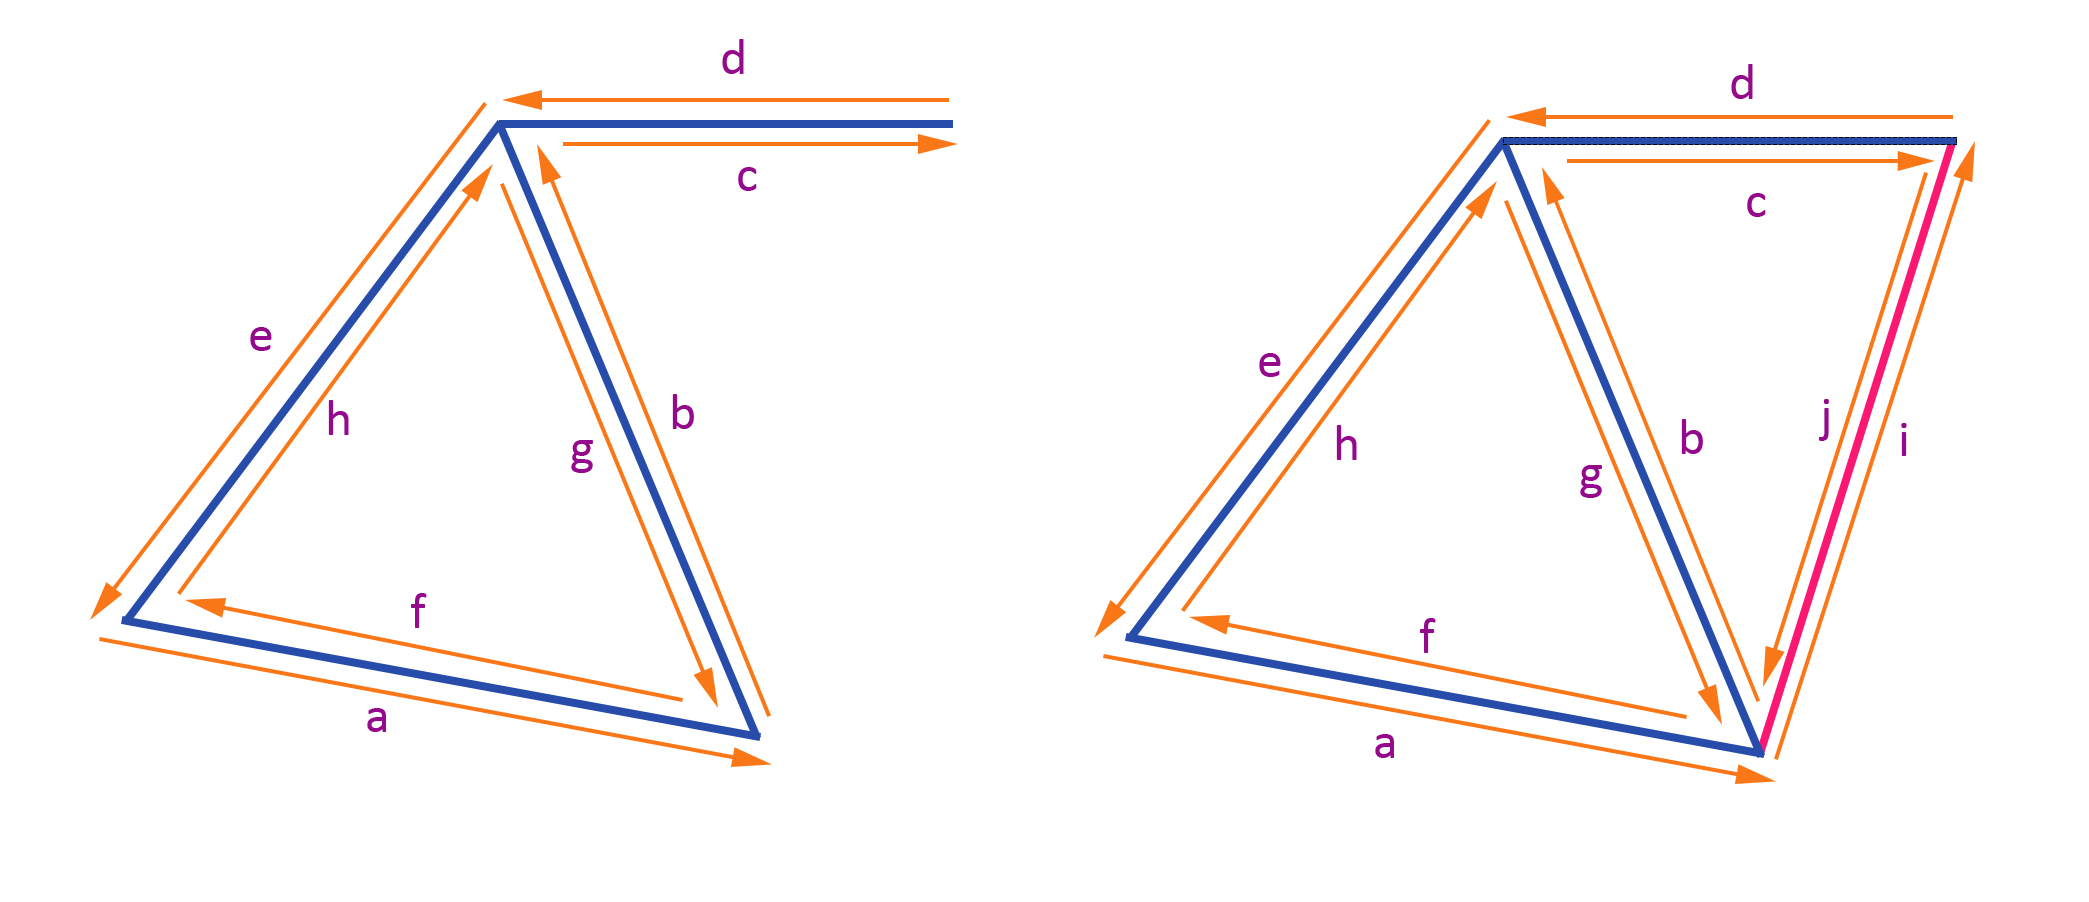
\includegraphics{Add edge HE.jpg}
          \caption{Agregar un arco a una estructura \textit{Half-edge}.}
          \label{fig:he-add-edge}
        \end{figure}
      
      \item Implemente un método para remover un arco entre dos vértices. 
        De manera similar a la pregunta anterior, esto implicará cambiar las referencias 
        de algunos de los semi-arcos.
      
      \item Agregue un método para remover un vértice de la estructura. 
        La eliminación de un vértice implica remover todos los semi-arcos conectados a 
        éste.
        
        \textit{Hint: utilice la solución de la pregunta anterior para eliminar los 
        arcos.}
    \end{enumerate}
  \end{Exercise}
%